% Source for diagram_01.svg — linear classification in feature space.
% Regenerate with:
%   pdflatex diagram_01.tex && inkscape --export-plain-svg -o diagram_01.svg diagram_01.pdf
\documentclass[tikz,border=4pt]{standalone}
\usepackage{amsmath}
\begin{document}
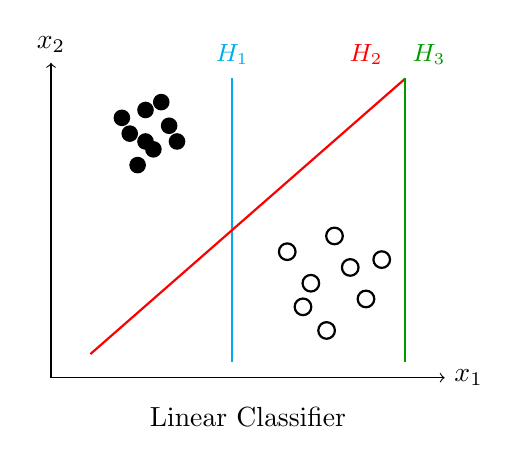
\begin{tikzpicture}[scale=1.0]
    % Axes
    \draw[->] (0,0) -- (5,0) node[right] {$x_1$};
    \draw[->] (0,0) -- (0,4) node[above] {$x_2$};

    % Class 1 (filled circles) - upper left cluster
    \foreach \x/\y in {0.9/3.3, 1.2/3.0, 1.4/3.5, 1.1/2.7, 1.5/3.2, 1.3/2.9, 1.0/3.1, 1.6/3.0, 1.2/3.4} {
        \fill[black] (\x,\y) circle (3pt);
    }

    % Class 2 (empty circles) - lower right cluster
    \foreach \x/\y in {3.0/1.6, 3.3/1.2, 3.6/1.8, 3.2/0.9, 3.8/1.4, 3.5/0.6, 4.0/1.0, 4.2/1.5} {
        \draw[black, thick] (\x,\y) circle (3pt);
    }

    % H1 (cyan) - vertical line in CENTER
    \draw[thick, cyan] (2.3,3.8) -- (2.3,0.2);

    % H2 (red) - diagonal from bottom-left to top-right
    \draw[thick, red] (0.5,0.3) -- (4.5,3.8);

    % H3 (green) - vertical line on far RIGHT
    \draw[thick, green!60!black] (4.5,3.8) -- (4.5,0.2);

    % Labels at top
    \node[cyan] at (2.3, 4.1) {\small $H_1$};
    \node[red] at (4.0, 4.1) {\small $H_2$};
    \node[green!60!black] at (4.8, 4.1) {\small $H_3$};

    % Title
    \node at (2.5, -0.5) {Linear Classifier};
\end{tikzpicture}
\end{document}
